
このチュートリアルでは,Fig. \ref{fig:domain}に示した
日本域を対象とした現実大気実験を行う.

SCALE-LESモデルの実行過程は,Fig. \ref{fig:howto}に示されるように
\begin{enumerate}
\item pp : 地形・海陸分布データの作成(現実大気実験のみ)
\item init : 初期値・境界値データの作成
\item run : 時間積分を行う(モデル本体の実行)
\end{enumerate}
といった手順で実行する.


\begin{figure}[h]
\begin{center}
  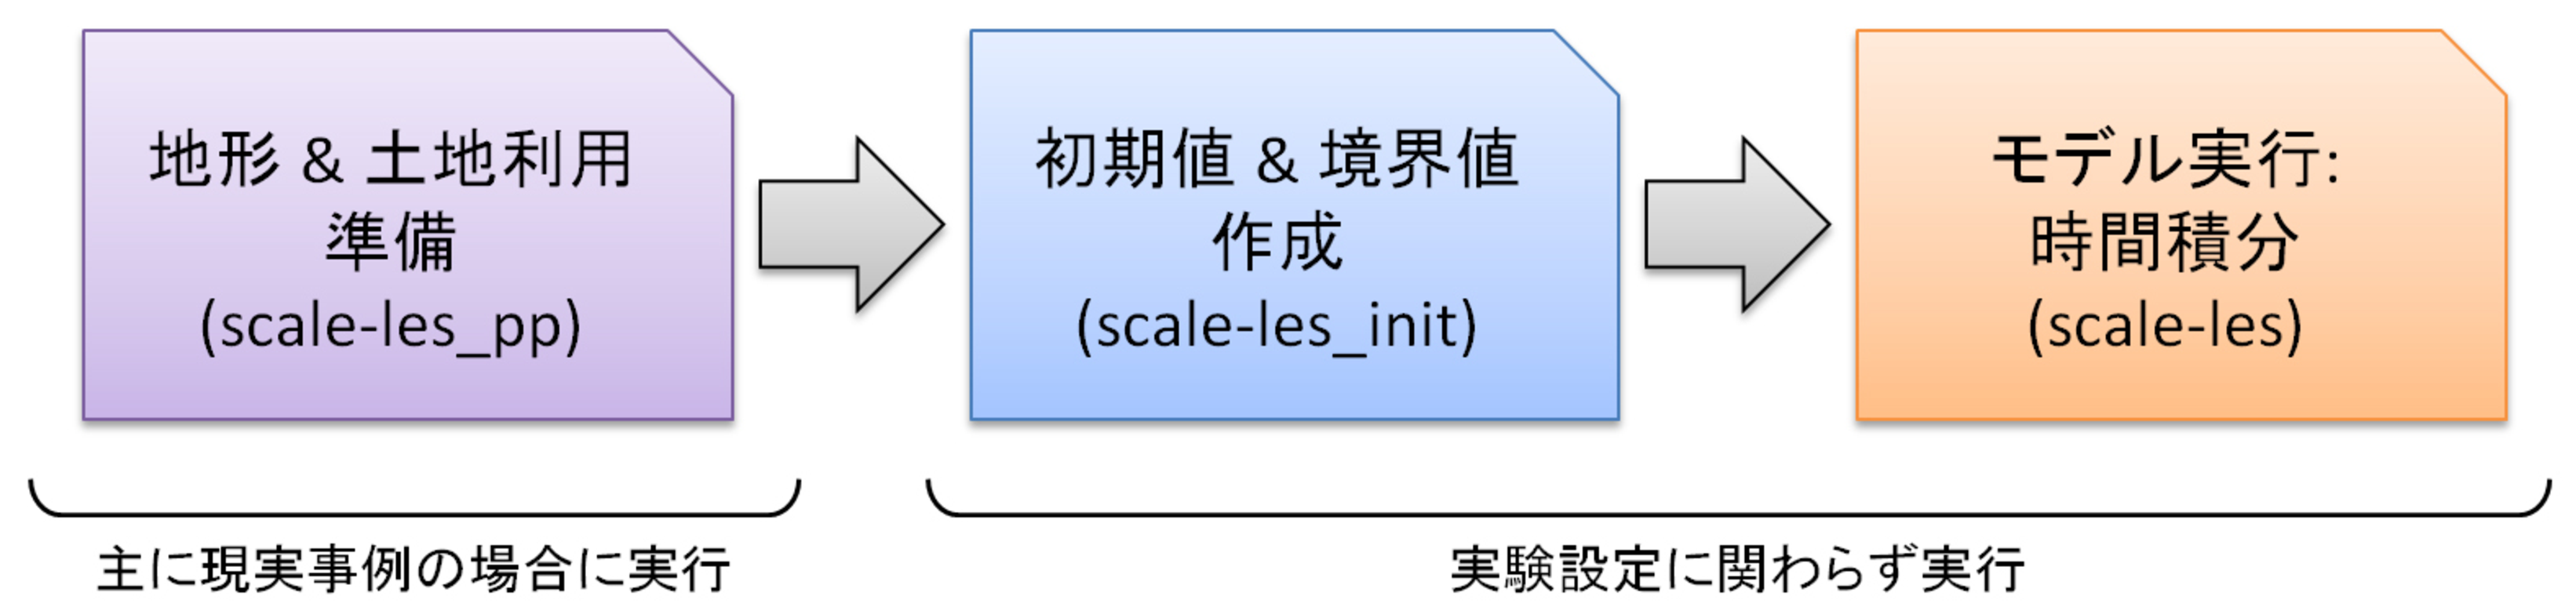
\includegraphics[width=0.9\hsize]{./figure/how_to_run.eps}\\
  \caption{SCALE-LESモデルの実行過程}
  \label{fig:howto}
\end{center}
\end{figure}

計算領域(ドメイン)の設定はTable \ref{tab:grids}のようになっている.

\begin{figure}[h]
\begin{center}
  \includegraphics[width=0.5\hsize]{./figure/domain.eps}\\
  \caption{計算領域.コンターは海岸線,カラーシェードは地形の高度を示す.}
  \label{fig:domain}
\end{center}
\end{figure}

\begin{table}[h]
\begin{center}
  \caption{実験設定の概略}
  \label{tab:grids}
  \begin{tabularx}{150mm}{|l|X|} \hline
    \rowcolor[gray]{0.9} 項目 & 設定 \\ \hline
    MPIプロセス分割 (東西 x 南北) & 2 x 2 (合計4プロセス) \\ \hline
    水平格子数 (東西 x 南北) & 60格子点 x 60格子点 \\ \hline
    鉛直層数                 & 36層                  \\ \hline
    水平格子間隔             & dx = dy = 15km       \\ \hline
    積分期間 & 2014年8月10日 00UTC~12UTC (12時間積分) \\ \hline
    時間ステップ間隔 & 30 sec (1440 steps) \\ \hline
  \end{tabularx}
\end{center}
\end{table}

%-------------------------------------------------------%
\section{境界データの入手: AICS内部用}
%-------------------------------------------------------%

現実大気実験を行う場合,SCALE本体に加えて境界値データが必要になる.
本チュートリアル用の気象場のデータ,日本領域の地形・土地利用のデータを\\
 \url{http://scale.aics.riken.jp/download/tutorial_data.tar.gz}\\
より入手し,チュートリアルの入力ファイル用ディレクトリ
\begin{verbatim}
  scale/scale-les/test/tutorial/data/
\end{verbatim}
の下に展開しておく.

以降の説明で\verb|${TOPDIR}|は,\verb|scale/scale-les/test/tutorial/|がある絶対PATHを指す.

\begin{verbatim}
  ${TOPDIR}/data/tutorial_data/input_atom/    <- 気象場データ
  ${TOPDIR}/data/tutorial_data/input_topo/    <- 地形データ
  ${TOPDIR}/data/tutorial_data/input_landuse/ <- 土地利用データ
\end{verbatim}
\verb|tutorial_data/|には,本チュートリアルに必要な最低限のデータのみが納めされているため,
その他の設定で実験を行う場合には別途,気象場,地形,および土地利用データが必要となる.


%-------------------------------------------------------%
\section{境界データの準備: 一般ユーザー用、公開時タイトル注意}
%-------------------------------------------------------%

現実大気実験のシミュレーションを行う場合,SCALE本体に加えて
境界値データが必要になる。境界値データとしては下記が必要である。
\begin{itemize}
\item 標高データ
\item 土地利用データ
\item 大気・地表面データ
\end{itemize}

ここでは、ユーザーが全球の任意の地域を対象とした計算できるよう、
標高データはUSGS(U.S. Geological Survey) のGTOPO30、
土地利用データはGLCCv2、
大気・地表面データはNCEP FNL(Final) Operational Global Analysis data
を用いる。
チュートリアルは、SCALEの使い方を学ぶことが目的であり、
ノートPCでも動く程度の軽い設定にしている。
領域モデルの実験設定として必ずしも適切な設定を選択しているわけではないので
ご留意頂きたい(例えば、スピンナップや領域など)。


\subsubsection{地形データと土地利用データ}

SCALE用の地形・土地利用のデータを\\
 \url{http://scale.aics.riken.jp/download/scale_database.tar.gz}\\
より入手し、任意のディレクトリー下に展開しておく。
makeを使ったjob scriptを使用する場合には、
展開先のディレクトリを SCALE\_DB という環境変数に設定しておくと便利である。
\begin{verbatim}
  $ tar -zxvf scale_database.tar.gz
  $ export SCALE_DB=${path_to directory_of_scale_database}/scale_database
\end{verbatim}
展開したディレクトリには、地形データと土地利用データが格納されている。
\begin{verbatim}
  ${SCALE_DB}/topo/    <- 地形データ
  ${SCALE_DB}/landuse/ <- 土地利用データ
\end{verbatim}


\subsubsection{大気・陸面データ}
\begin{enumerate}
\item データのダウンロード\\
NCARのサイト
 \url{http://rda.ucar.edu/datasets/ds083.2/}\\
から、2014年8月10日の00Z, 06Z, 12Z のデータ
\begin{verbatim}
  fnl_20140810_00_00.grib2
  fnl_20140810_06_00.grib2
  fnl_20140810_12_00.grib2
\end{verbatim}
を任意のディレクトリ(以後、\verb|${FNL_dir}|と表記)の
\verb|org|以下にダウンロードする.

\item データフォーマットをgribからbinaryに変換\\
SCALEは4byte バイナリー(grads format)の境界値データを
読み込むことができる。
\verb|${FNL_dir}|の下に、\verb|tutrial/tools/convert_grib2grads.sh|をコピー。
\begin{verbatim}
  $ cp tutrial/tools/convert_grib2grads.sh ${FNL_dir}/
\end{verbatim}
そして、実行する。
\begin{verbatim}
  $ sh convert_grib2grads.sh
\end{verbatim}
成功すれば、下記のファイルが作成される。
\begin{verbatim}
  $ ls FNL_output/*/*
     FNL_output/201408/FNL_2014081000.grd
     FNL_output/201408/FNL_2014081006.grd
     FNL_output/201408/FNL_2014081012.grd
\end{verbatim}
\end{enumerate}

